\documentclass[12pt, oneside]{article}
\usepackage[letterpaper, margin=1in, headsep=0.5in]{geometry}
\usepackage[english]{babel}
\usepackage[utf8]{inputenc}
\usepackage{amsmath}
\usepackage{amsfonts}
\usepackage{amssymb}
\usepackage{tikz}
\usetikzlibrary{quotes, angles}
\usepackage{graphicx}
%\usepackage{pgfplots}
%\pgfplotsset{width=10cm,compat=1.9}
%\usepgfplotslibrary{statistics}
%\usepackage{pgfplotstable}
%\usepackage{tkz-fct}
%\usepackage{venndiagram}
\usepackage{multicol}


\usepackage{fancyhdr}
\pagestyle{fancy}
\fancyhf{}
\rhead{\thepage \\Name: \hspace{1.5in}.\\}
\lhead{BECA / Dr. Huson / Geometry 10th Grade\\* Unit 4: Triangle Congruence\\30 November 2018}

\renewcommand{\headrulewidth}{0pt}

\begin{document}
\subsubsection*{Take-home Test}
Open book, open notes. You may use your notebook, papers, and online resources. No working with classmates or other human help.

\begin{enumerate}

  \item Given $m\angle E=44$, and $m\angle GFH=112$. Find $m\angle G$.\\[1cm]
    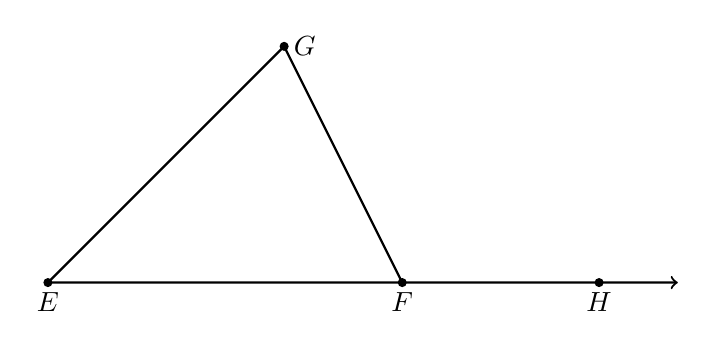
\begin{tikzpicture}
      %\draw [->, thick] (0,0)--(5,5);
      \draw [<-, thick] (8,0)--(0,0)--(3,3)--(4.5,0);
      \draw [fill] (0,0) circle [radius=0.05] node[below]{$E$};
      \draw [fill] (4.5,0) circle [radius=0.05] node[below]{$F$};
      \draw [fill] (3,3) circle [radius=0.05] node[right]{$G$};
      \draw [fill] (7,0) circle [radius=0.05] node[below]{$H$};
    \end{tikzpicture}
    \vspace{4cm}

  \item Given two vertical angles, $m \angle 1 = 4x+5$, $\displaystyle m \angle 2 = \frac{9x-7}{2}$. Find $m \angle 1$.\\
  For full credit, check by comparing to $m\angle 2$.
      \begin{flushright}
      \begin{tikzpicture}[scale=.7]
        \draw [<->, thick] (0,-1.5)--(10,1.5);
        \draw [<->, thick] (2,3.5)--(7,-3.5);
        \node at (3,.4){1};
        \node at (6,-.6){2};
      \end{tikzpicture}
      \end{flushright}

\newpage
  \item Given the situation in the diagram, answer each question. Circle True or False. %\vspace{1cm}
      \begin{center}
      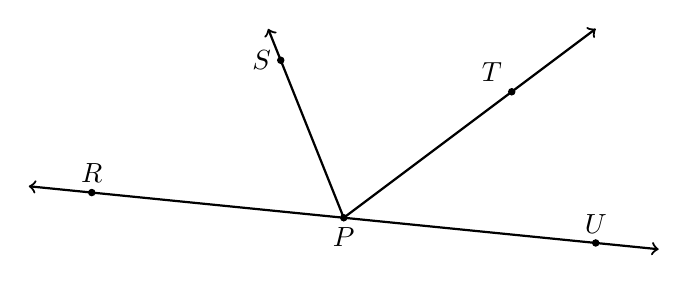
\begin{tikzpicture}[scale=0.8]
        \draw [->, thick] (0,0)--(4,3);
        \draw [<->, thick] (-5,.5)--(5,-.5);
        \draw [->, thick] (0,0)--(-1.2,3);
        \draw [fill] (-1,2.5) circle [radius=0.05] node[left ]{$S$};
        \draw [fill] (2.66666,2) circle [radius=0.05] node[above left ]{$T$};
        \draw [fill] (0,0) circle [radius=0.05] node[below]{$P$};
        \draw [fill] (4,-0.4) circle [radius=0.05] node[above]{$U$};
        \draw [fill] (-4,0.4) circle [radius=0.05] node[above]{$R$};
      \end{tikzpicture}
    \end{center}
    \begin{enumerate}
      \item True or False: $\angle SPU$ is an obtuse angle.
      \item True or False: $\overrightarrow{SP}$ and $\overrightarrow{PS}$ are opposite rays.
      \item True or False: $\angle RPT$ and $\angle TPU$ are a linear pair.
      \item True or False: $\angle SPT$ and $\angle RPS$ are adjacent.
    \end{enumerate}

  \item Given two parallel lines and a transversal, as shown. Apply the theorem, ``If a transversal intersects two parallel lines, then corresponding angles are congruent."
    \begin{center}
    \begin{tikzpicture}
      \draw [<->, thick] (1,2)--(9,2);
      \draw [<->, thick] (0,0)--(8,0);
      \draw [<->, thick] (4,-1)--(5.5,3);
      \node at (4.5,0.3) [left]{$5$};
      \node at (4.5,0.3) [right]{$6$};
      \node at (4.3,-0.3) [left]{$7$};
      \node at (4.3,-0.3) [right]{$8$};
      \node at (5.2,2) [above left]{$1$};
      \node at (5.2,2) [above right]{$2$};
      \node at (5,2) [below left]{$3$};
      \node at (5,2) [below right]{$4$};
    \end{tikzpicture}
    \end{center}
    \begin{enumerate}
      \item State the angle corresponding with $\angle 7$. \bigskip
      \item Given $m\angle 2 = 68^\circ$. Find $m\angle 3$. \bigskip
      \item In a proof, what reason would justify $\angle 4 \cong \angle 5$? \rule{6cm}{0.15mm} \bigskip
      \item Given $m\angle 5 = 112^\circ$ and $m\angle 3 = 4x^\circ$. Find $x$.
    \end{enumerate}

\newpage
  \item On the graph below, draw $\overline{CD}$, with $C(-1,6)$ and $D(7,3)$, labeling the end points. Determine and state the coordinates of the midpoint $M$ of $\overline{CD}$ and mark and label it on the graph.\\[0.5cm]
    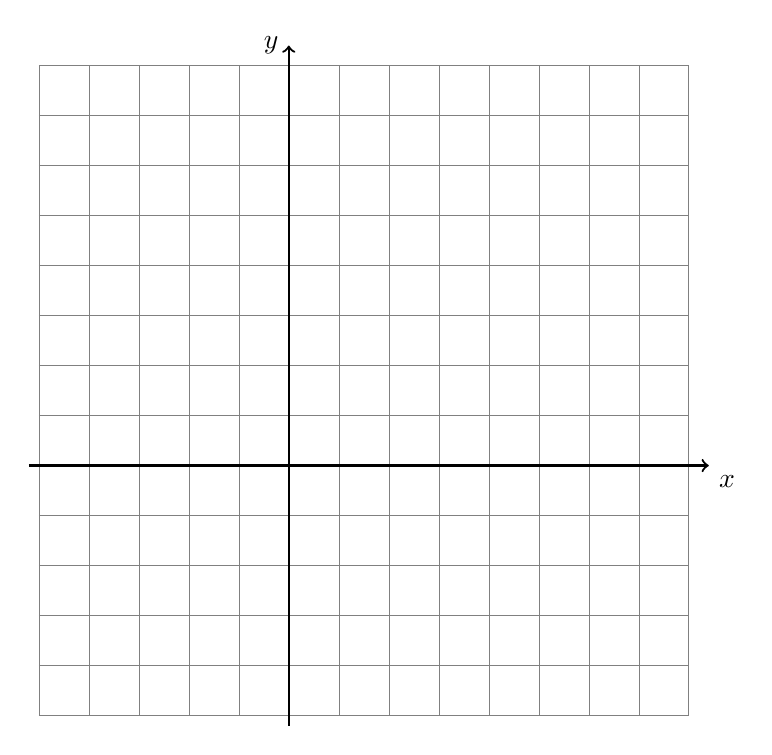
\begin{tikzpicture}[scale=.635]
      \draw [help lines] (-5,-5) grid (8,8);
      \draw [thick, ->] (-5.2,0) -- (8.4,0) node [below right] {$x$};
      \draw [thick, ->] (0,-5.2)--(0,8.4) node [left] {$y$};
    \end{tikzpicture}
    \vspace{2cm}

  \item Given $\overline{ABC}$, $AC=24$, and the point $B$ partitions $\overline{AC}$ in a ratio of 1:3.\\[0.5cm] Find ${AB}$. \\[1cm]
  \begin{center}
      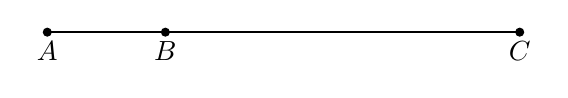
\begin{tikzpicture}
        \draw [-, thick] (1,0)--(7,0);
        \draw [fill] (1,0) circle [radius=0.05] node[below]{$A$};
        \draw [fill] (2.5,0) circle [radius=0.05] node[below]{$B$};
        \draw [fill] (7,0) circle [radius=0.05] node[below]{$C$};
      \end{tikzpicture}
    \end{center}
      \vspace{2cm}

\newpage

  \item Given $\overleftrightarrow{KM}$ as shown on the number line, with $K$ having the coordinate 2.2 and $M$ the coordinate 5.1 \\[10pt] % Midpoint
    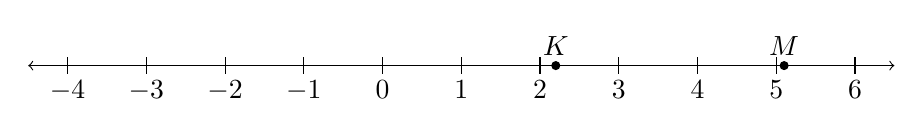
\begin{tikzpicture}
      \draw [<->] (-4.5,0)--(6.5,0);
      \foreach \x in {-4,...,6} %2 leading for diff!=1
        \draw[shift={(\x,0)},color=black] (0pt,-3pt) -- (0pt,3pt) node[below=5pt]  {$\x$};
        \draw [fill] (2.2,0) circle [radius=0.05] node[above] {$K$};
        \draw [fill] (5.1,0) circle [radius=0.05] node[above] {$M$};
    \end{tikzpicture}
    \begin{enumerate}
      \item Find the value of the coordinate of the point $L$, the midpoint of $\overline{KM}$. \vspace{4cm}
      \item The point $J$ is collinear with $\overleftrightarrow{KM}$ such that $K$ is the midpoint of $\overleftrightarrow{JM}$. Mark $J$ on the line and state the value of its coordinate.
    \end{enumerate} \vspace{3cm}

  \item Given $\triangle DEF$. $\overline{DF} \cong \overline{EF}$,  $m\angle F=68$. Find $m\angle D$.\\[0.5cm]
    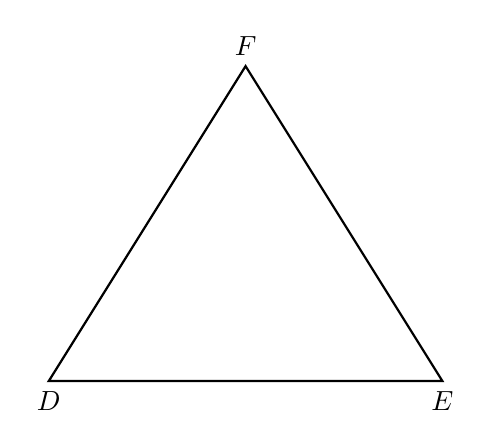
\begin{tikzpicture} %[scale=3] Isosceles, parallel marks, congruence marks
      \draw [-, thick] (0,0) node[below]{$D$}--
        (5,0) node[below]{$E$}--(2.5,4) node[above]{$F$}--cycle;
      %\draw [>->, thick] (1.0,1.6)--(1.25,2);
      %\draw [{Bar[]}-{Bar[]}, thick] (4,1.6)--(3.75,2);
      %\draw [color=blue] (0.75,0) arc [start angle=0, end angle=58, radius=0.75];
      %\draw (5,0)-- +(-0.75,0) arc [start angle=180, end angle=122, radius=0.75];
    \end{tikzpicture}%\vspace{1cm}

\newpage

  \item Construct a duplicate of the given angle $A$.  [Leave all construction marks.]\\[2cm]
      \begin{tikzpicture}
        \draw [<->, thick] (3,5)--(0,0)--(6,0);
        \draw [fill] (0,0) circle [radius=0.05] node[below]{$A$};
        %\draw [fill] (7,0) circle [radius=0.05] node[below]{$N$};
      \end{tikzpicture}
      \vspace{2cm}

  \item Construct a perpendicular to $\overline{AB}$ through $C$.\\
    %\hspace{1cm} Given the line  $l$ and point $P$.
    \vspace{2cm}
    \begin{center}
    \begin{tikzpicture}
      \draw [<->, thick] (0,0)--(11,0)--(7,3)--cycle;
      \draw [fill] (0,0) circle [radius=0.05] node[left]{$A$};
      \draw [fill] (11,0) circle [radius=0.05] node[right]{$B$};
      \draw [fill] (7,3) circle [radius=0.05] node[above right]{$C$};
    \end{tikzpicture}
    \end{center}


\newpage
  \item Construct the angle bisectors of the angles of the triangle and their intersection, the incenter.\\
    %\hspace{1cm} Given the line  $l$ and point $P$.
    \vspace{3cm}
    \begin{center}
    \begin{tikzpicture}[scale=1.2]
      \draw [<->, thick] (0,0)--(9,0)--(7,11)--cycle;
      %\draw [fill] (2,3) circle [radius=0.05] node[right]{$P$};
      %\node at (8.5,-0.4){$l$};
      %\draw [fill] (6,0) circle [radius=0.05] node[below]{$Q$};
    \end{tikzpicture}
    \end{center}

\newpage

\item Construct the centroid of $\triangle ABC$, leaving all construction marks.
  \vspace{5cm}
  \begin{center}
  \begin{tikzpicture}[scale=1.2]
    \draw [<->, thick] (0,0)--(6.5,0)--(6,4)--cycle;
    \draw [fill] (0,0) circle [radius=0.05] node[left]{$A$};
    \draw [fill] (6.5,0) circle [radius=0.05] node[right]{$B$};
    \draw [fill] (6,4) circle [radius=0.05] node[above right]{$C$};
  \end{tikzpicture}
\end{center} \vspace{1.5cm}

\newpage

  \item Given $M(-7,10)$ and $N(-2,-2)$, find the length of $\overline{MN}$.
      \vspace{5cm}

  \item Given $\triangle GEM$ with $G(-9, -3)$, $E(6, -3)$, and $M(6, 5)$.
    \begin{enumerate}
      \item Plot and label $\triangle GEM$ on the graph, labeling its vertices.
      \item Find the lengths of each side of the triangle. Show the substitution into the proper formulas for full credit.
    \end{enumerate}
    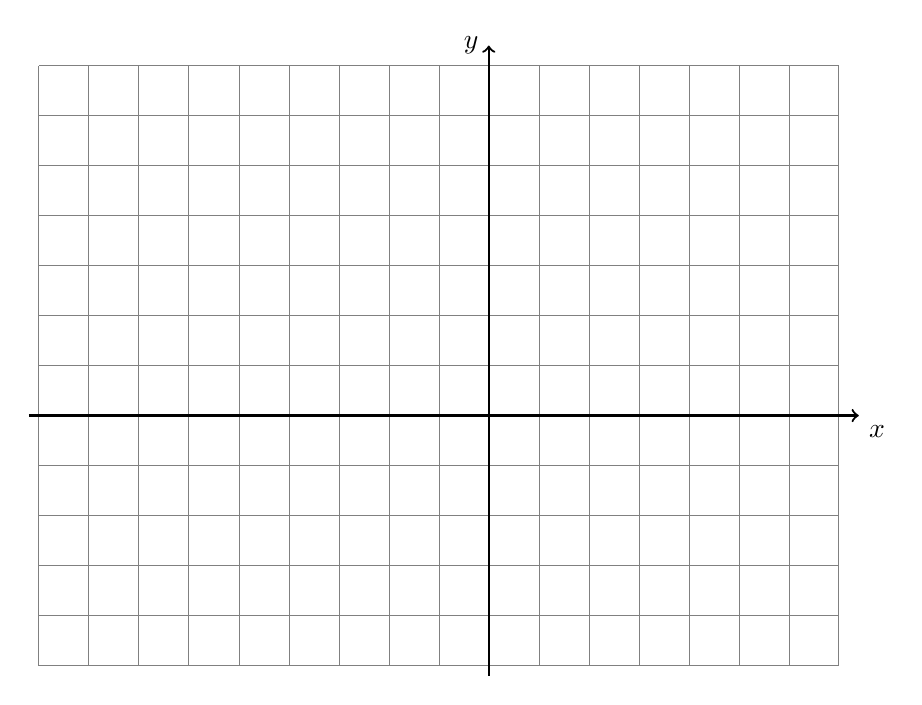
\begin{tikzpicture}[scale=.635]
      \draw [help lines] (-9,-5) grid (7,7);
      \draw [thick, ->] (-9.2,0) -- (7.4,0) node [below right] {$x$};
      \draw [thick, ->] (0,-5.2)--(0,7.4) node [left] {$y$};
    \end{tikzpicture}
    \vspace{3cm}


\newpage
\item Given right $\triangle EFG$ with $m\angle G=90^\circ$, $EG=8$, and $m\angle E=43^\circ$. Express each trig ratio as a fraction.  \vspace{0.5cm}
\begin{multicols}{2}
  \begin{enumerate}
    \item $\sin E=$ \vspace{0.8cm}
    \item $\tan E=$ \vspace{0.8cm}
    \item Find $EF$.
  \end{enumerate}
  \begin{center}
    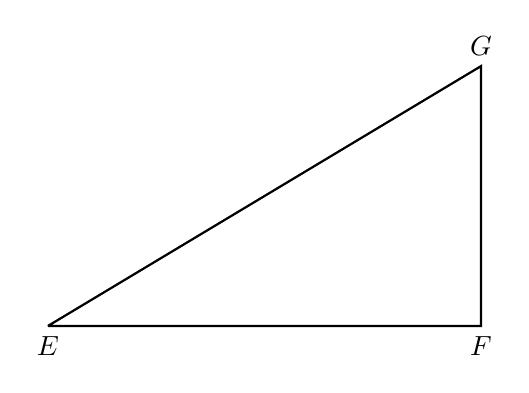
\begin{tikzpicture}[scale=1.1]
      \draw [thick]%(0,0)node[below]{$A$}--
        (0,0)node[below]{$E$}--
        (5,0)node[below]{$F$}--
        (5,3)node[above]{$G$} --(0,0);
    \end{tikzpicture}
      \vspace{2cm}
  \end{center}
\end{multicols}
\vspace{3cm}

  \item Find the slope of each line.
  \begin{multicols}{2}
    \begin{enumerate}
      \item $y=-3x-7$
      \item $2x-3y=9$
    \end{enumerate}
  \end{multicols} \vspace{3cm}

  \item Find the slope of the line through the points $A(5,3)$ and $B(7,-1)$. \vspace{3cm}

\newpage

  \item Given the quadrilateral $RSTU$ with $R(-8,-1)$, $S(2,-1)$, $T(10,5)$, and $U(0,5)$.
  \begin{enumerate}
    \item Plot and label $RSTU$ on the grid.
    \item Find the slope of the diagonals $\overline{RT}$ and $\overline{SU}$.
    \item Theorem: A quadrilateral is a rhombus if and only if its diagonals are perpendicular.\\[0.5cm]
    Prove that $RSTU$ is a rhombus.
  \end{enumerate}

  \begin{center} %4 quadrant regents grid w T-Chart
  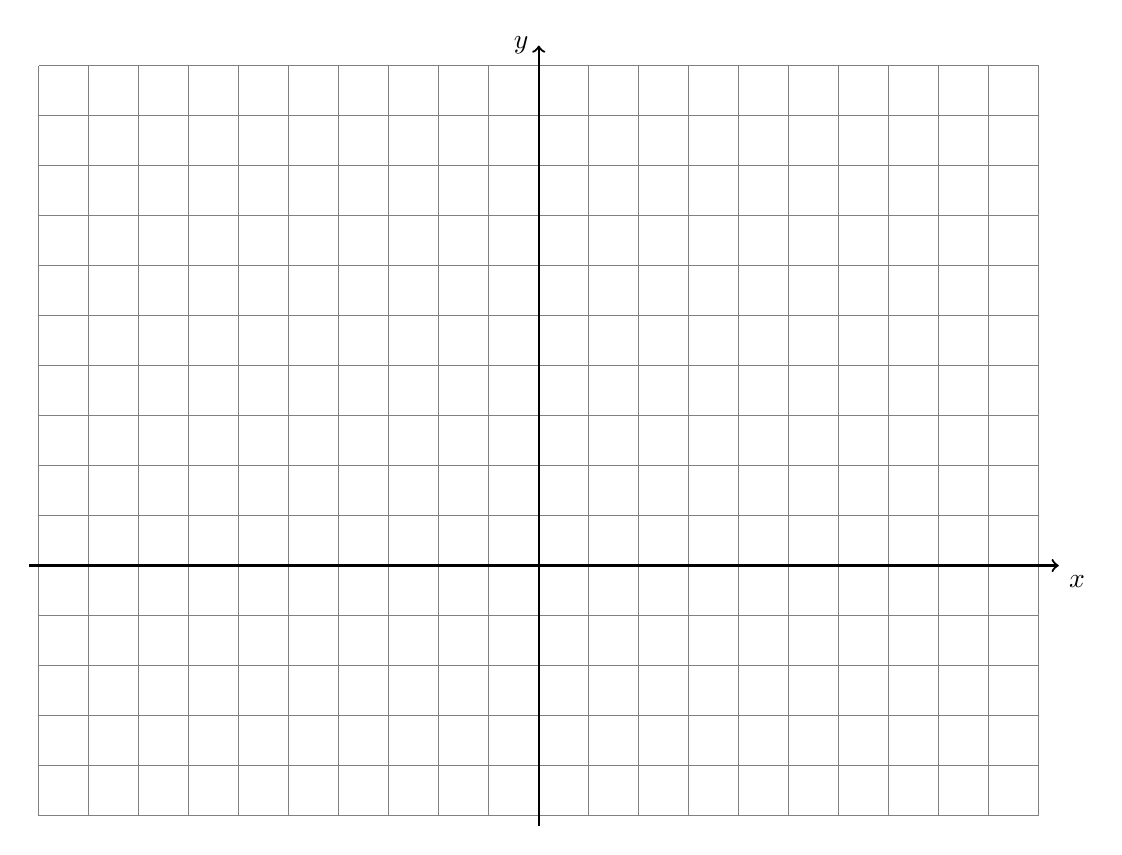
\begin{tikzpicture}[scale=.635]
    \draw [help lines] (-10,-5) grid (10,10);
    \draw [thick, ->] (-10.2,0) -- (10.4,0) node [below right] {$x$};
    \draw [thick, ->] (0,-5.2)--(0,10.4) node [left] {$y$};
  \end{tikzpicture}
  \end{center}

\newpage

  \item Given the square $EASY$ with $E(-1, 1)$, $A(6, 1)$, $S(6, 8)$, and $Y(-1, 8)$.
    \begin{enumerate}
      \item Draw $EASY$ on the graph, labeling the vertices.
      \item Find the area of $EASY$. \vspace{2cm}
      \item Find the perimeter of $EASY$. \vspace{2cm}
    \end{enumerate}
      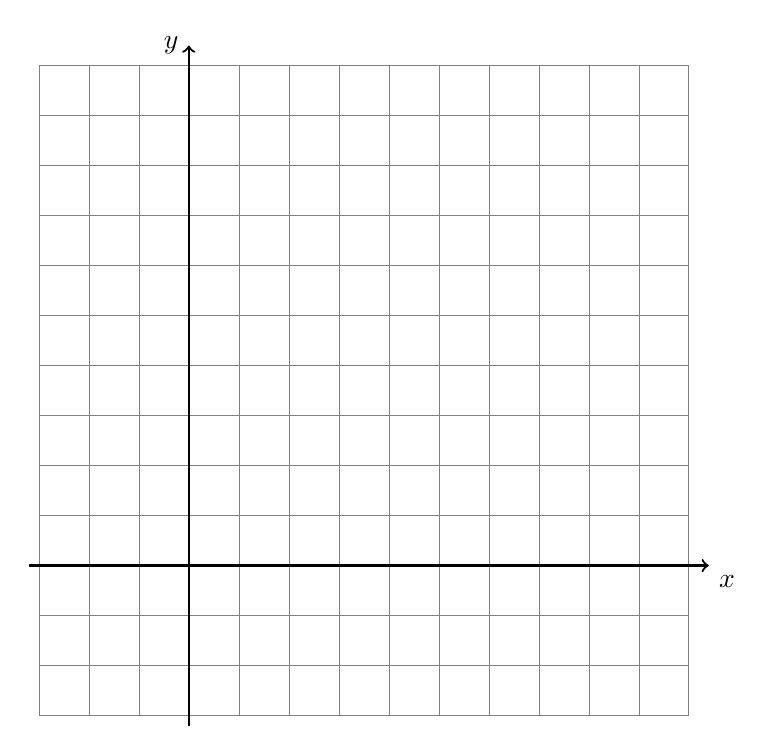
\begin{tikzpicture}[scale=.635]
        \draw [help lines] (-3,-3) grid (10,10);
        \draw [thick, ->] (-3.2,0) -- (10.4,0) node [below right] {$x$};
        \draw [thick, ->] (0,-3.2)--(0,10.4) node [left] {$y$};
      \end{tikzpicture}

  \item Given a circle $O$ with radius $2.2$.
  \begin{enumerate}
    \item Find the circumference of $O$. \vspace{2cm}
    \item Find the area of $O$.
  \end{enumerate}

\newpage

  \item Given the circle $C$ with circumference $8\pi$.
  \begin{enumerate}
    \item Write down the formula for the circumference of a circle and solve for the radius yielding a circumference of $8\pi$. \vspace{1cm}
    \item Find the area of the circle.
  \end{enumerate}
  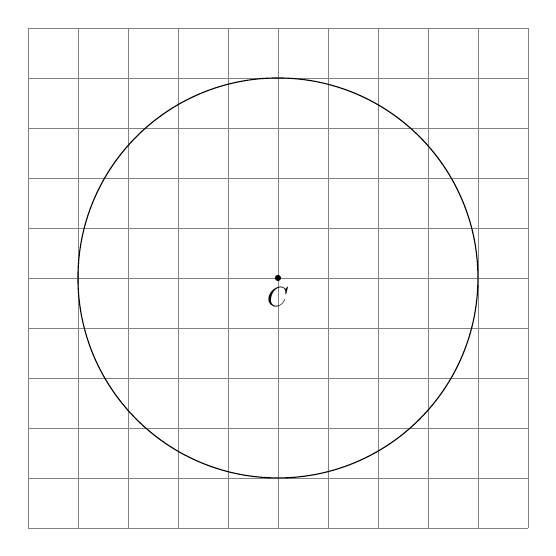
\begin{tikzpicture}[scale=.635]
    \draw [help lines] (-5,-5) grid (5,5);
    %\draw [thick, ->] (-2.2,0) -- (10.4,0) node [below right] {$x$};
    %\draw [thick, ->] (0,-2.2)--(0,10.4) node [left] {$y$};
    \draw (0,0) circle [radius=4] node[below]{$C$};
    \draw [fill] (0,0) circle [radius=0.05];
  \end{tikzpicture}

  \item On the graph, draw polygon ABCDEF with vertices A(-1, 1), B(4, 1),
  C(4, 5), \\ D(9, 5), E(9, 8), and F(-1, 8). Find the perimeter and the area of the polygon.\\[1cm]
  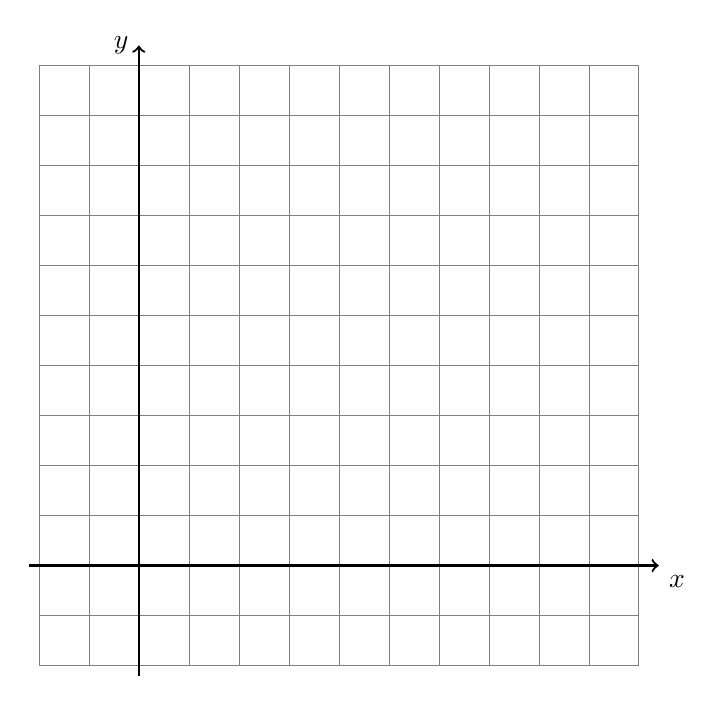
\begin{tikzpicture}[scale=.635]
    \draw [help lines] (-2,-2) grid (10,10);
    \draw [thick, ->] (-2.2,0) -- (10.4,0) node [below right] {$x$};
    \draw [thick, ->] (0,-2.2)--(0,10.4) node [left] {$y$};
  \end{tikzpicture}
  \vspace{2cm}



  \end{enumerate}

\end{document}
